\chapter{Two shortcomings of Korat}
\label{ch:shortcomings-of-korat}
This chapter presents two example scenarios where
Korat fails to perform as expected.  The first
example shows how the use of reflection for field accesses may render
Korat unable to generate some valid structures.  The second example
shows how a poorly-written \emph{RepOk} may adversely affect the performance
of Korat and force it to explore many more states than necessary.
Both examples use a binary tree data structure and implement different
\emph{RepOk} methods that check the same set of properties but operate
differently.  We compare the performance of Korat by using these \emph{RepOk}
methods against using the standard binary tree RepOk from Korat
distribution.  Chapter~\ref{ch:evaluation} provides experimental
results using additional data structures.

\section{Usage of reflection for field access}
\label{sec:usage-of-reflection-for-field-access}
This example first illustrates how a \emph{RepOk} method can be written with
and without using reflection for field accesses and then shows how the
output of Korat differs in terms of the sets of valid structures
generated.

\para
Figure~\ref{fig:btreeDirectRepOk} shows the Java declaration of a
binary tree and a standard implementation of its \emph{RepOk}
method\footnote{\url{korat.sourceforge.net}}. Each object of the class
\emph{BinaryTree} represents a binary tree. The value of the
\emph{size} field is the number of nodes in the tree. Objects of the
inner class \emph{Node} represent nodes of the tree.  The \emph{RepOk} method
performs a traversal of its input object graph and checks that it has
no cycle and the value of the size field is correctly set to the
actual number of nodes reachable from root.  In more detail, first,
\emph{RepOk} checks if the tree is empty. If not, \emph{RepOk} checks
that there are no undirected cycles in the object graph reachable from
the \emph{root} field along the \emph{left} and \emph{right}
fields. It finally checks that the number of nodes reachable from the
root is the same as the value of field \emph{size}.

\begin{figure}
\centering
\begin{lstlisting}[language=Java]
class BinaryTree {
    Node root;    // root node
    int size;    // number of nodes in the tree
    static class Node {
        Node left;    // left child
        Node right;    // right child
    }

    boolean RepOk() {
        // checks that empty tree has size zero.
        if (root == null) return size == 0;
        Set visited = new HashSet();
        visited.add(root);
        LinkedList workList = new LinkedList();
        workList.add(root);
        // loop checks that the object graph is a tree.
        while (!workList.isEmpty()) {
            Node current = (Node) workList.removeFirst();
            if (current.left != null) {
                if (!visited.add(current.left))
                    return false;
                workList.add(current.left);
            }
            if (current.right != null) {
                if (!visited.add(current.right))
                    return false;
                workList.add(current.right);
            }
        }
        // checks that the size is consistent.
        return (visited.size() == size);
    }
}
\end{lstlisting}
\caption{Binary tree example with RepOk using direct field access.}
\label{fig:btreeDirectRepOk}
\end{figure}

\para
Recall, to bound the number of structures generated by Korat, the
programmer provides a finitization that specifies bounds on the number
of objects for different types in the data structures and on the
values in the fields of these objects.  For our binary tree example,
the finitization specifies the maximum number of nodes.  A tree is
considered to be in \emph{scope} $n$, if it has at most $n$ nodes. We
can use integers from 0 to $n$ for the \emph{size} field inside the
\emph{BinaryTree} class.

\para Recall also, given a finitization and a value for scope, Korat
generates all non-isomorphic structures that exist for the scope.  In
our example, two binary trees are isomorphic if a permutation of nodes
exists such that it maps each binary tree to the other.

\begin{figure}
\centering
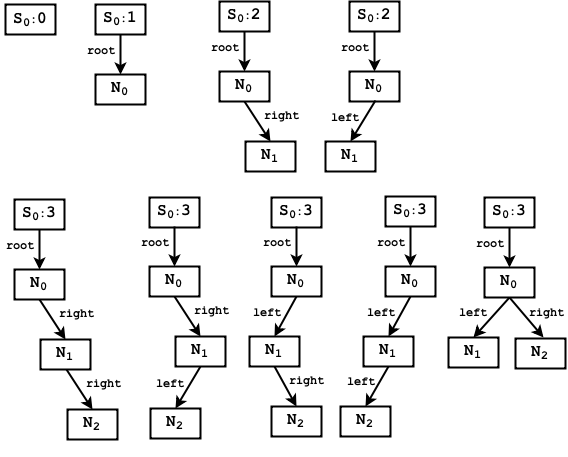
\includegraphics[width=12cm,height=8cm,keepaspectratio]{korat_instances_binary_tree_size_3}
\caption{Binary trees that Korat generates for scope three.}
\label{fig:btreeKoratGenScopeThree}
\end{figure}

\para When using the \emph{RepOk} shown in Figure~\ref{fig:btreeDirectRepOk} with a scope of three, the Korat search
evaluates 90 non-isomorphic candidate structures and outputs 9
structures, which are valid since they satisfy the \emph{RepOk}.
Figure~\ref{fig:btreeKoratGenScopeThree} shows the trees that Korat
generates for scope three. Each tree consists of one \emph{BinaryTree}
object $S_0$ and upto three \emph{Node} objects ($N_0$, $N_1$,
$N_2$). For each object, the value and the identity of the \emph{Node}
objects is shown. Edges represent the values of reference fields with
no edge for \emph{null}.


\para To enable efficient search for valid structures, Korat encodes
each structure using a \emph{candidate vector}, which represents the
\emph{state} of Korat's backtracking search; the finitization defines
the \emph{bounded state space}.  For each candidate that Korat
explores, it translates the candidate to a Java object graph and
invokes \emph{RepOk} on the resulting object.  Korat monitors these
executions to dynamically determine which fields of the candidate are
accessed by \emph{RepOk} before returning its result.  Korat monitors field
accesses by using bytecode instrumentation to replace them with
accessor methods that notify an observer of the accesses. If the
predicate returns \emph{true}, Korat outputs the candidate as a valid
structure for testing. Otherwise, if the predicate returns false,
Korat does not output the candidate.  When RepOk terminates, Korat
creates the next candidate based on the fields accessed during the
\emph{RepOk's} last execution.  Specifically, Korat tries the next value for
the last field accessed (based on the time of first access) to
systematically explore the state space.  Backtracking based on last
field access allows Korat to prune effectively; moreover Korat defines
non-isomorphic generation to further prune from consideration
candidates that are isomorphic to previously explored candidates.  If
all values for a field are exhausted, Korat backtracks to the previous
field, again based on the field-access order.  Korat terminates when
it has explored the entire search space (of course with pruning).

\begin{figure}
\centering
\begin{lstlisting}[language=Java]
//use of reflection might throw an exception
boolean repOK() throws Exception{
    // checks that empty tree has size zero.
    if (root == null) return size == 0;
    Set visited = new HashSet();
    visited.add(root);
    LinkedList workList = new LinkedList();
    workList.add(root);
    // loop checks that the object graph is a tree.
    while (!workList.isEmpty()) {
        Node current = (Node) workList.removeFirst();
        if ((Node)Node.class.getDeclaredField(``left'').get(current) != null) {
            if (!visited.add(current.left)) 
                return false;
            workList.add(current.left);
        }
        if (current.right != null) {
            if (!visited.add(current.right))
                return false;
            workList.add(current.right);
        }
    }
    // checks that the size is consistent.
    return (visited.size() == size);
}
\end{lstlisting}
\caption{RepOk using the java reflection API for accessing the left child of a Node inside the loop.}
\label{fig:btTreeReflectionRepOK}
\end{figure}


\begin{figure}
\centering
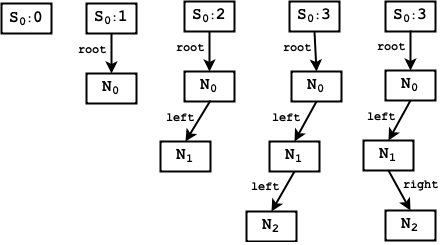
\includegraphics[width=11cm,height=6cm,keepaspectratio]{korat_instances_reflection_binary_tree_size_3}
\caption{ Binary trees that Korat generates for scope three when RepOk uses reflection.}
\label{fig:btreeReflectKoratGenScopeThree}
\end{figure}

Figure~\ref{fig:btreeDirectRepOk} illustrates the use of reflection
for field access.  Specifically, it shows the same \emph{RepOk} property
check as Figure~\ref{fig:btreeDirectRepOk} but with the use of
reflection: field access of left field of the node removed from the
\emph{workList} is using the Java reflection API instead of direct
field de-referencing.  The use of reflection renders Korat unable to
monitor the corresponding field(s) since Korat's monitoring is based
on actual field accesses (using \texttt{GETFIELD} bytecode
operations).  Given this reflection-based \emph{RepOk}
(Figure~\ref{fig:btreeDirectRepOk}), Korat evaluates only 28
non-isomorphic candidate structures of which 5 structures are output,
which are valid since they satisfy the \emph{RepOk};
Figure~\ref{fig:btreeReflectKoratGenScopeThree} illustrates these 5
structures.  Thus, the use of reflection reduces (1)~the state space
Korat explores simply because Korat is unable to create the \emph{data
  choices} appropriately and (2)~the number of valid candidates.  Note
however, since Korat never generates a candidate for which \emph{RepOk}
returns false, Korat only generates valid candidates even if
reflection is used.  Thus, reflection compromises completeness of
Korat's search (but not the soundness of the outputs generated).  Note
since the use of reflection may result in an exception, the \emph{RepOk} in
Figure~\ref{fig:btTreeReflectionRepOK} has a \texttt{throws} declaration.

\emph{RepOk} methods may use helper methods.  Korat instruments all the
helper methods, so it can monitor any fields they access.  However, as
before, if any helper method uses reflection, Korat cannot monitor
those accesses.

\section{Inefficient predicates}
\label{sec:inefficient-predicates}

Korat's pruning is sensitive to the way RepOk is written because
Korat's backtracking depends directly on the field accesses made by
\emph{RepOk}.  Thus, a poorly written \emph{RepOk}, e.g., one that accesses all
(reachable) fields regardless of whether the current structure is
already determined to be valid or invalid, may force Korat to consider
a very large number of candidate structures and perform poorly.  Note
that such poorly written \emph{RepOk's} do not force Korat to generate
incorrect an incorrect result, rather they degrade its performance.

\begin{figure}
\centering
\begin{lstlisting}[language=Java]
boolean repOK() {
    boolean result = true;
    // checks that empty tree has size zero.
    if (root == null) result = (size == 0);
    Set visited = new HashSet();
    LinkedList workList = new LinkedList();
    if (root != null) {
        visited.add(root);
        workList.add(root);
    }
    // loop checks that the object graph is a tree.
    while (!workList.isEmpty()) {
        Node current = (Node) workList.removeFirst();
        if (current.left != null) {
            if (!visited.add(current.left))
                result = false;
            else workList.add(current.left);
        }
        if (current.right != null) {
            if (!visited.add(current.right)) 
                result = false;
            else workList.add(current.right);
        }
    }
    // checks that the size is consistent.
    if(!result) result = (visited.size() == size);
    return result;
}
\end{lstlisting}
\caption{RepOk that does not return the result as soon as it is computed.}
\label{fig:bTreeInefficient}
\end{figure}

A standard guideline to increase Korat's efficiency is to write a
\emph{RepOk} that \emph{short-circuits} when possible, e.g., returns result
as soon as it is known.  Indeed, there can be significant
performance difference between a poorly-written and an optimized RepOk
as we illustrate next.

\para 
Recall, when using the \emph{RepOk} implementation shown in
Figure~\ref{fig:btreeDirectRepOk} with a scope of three, Korat
evaluates 90 non-isomorphic candidate structures of which 9 structures
are output. To contrast, consider the \emph{RepOk} implementation
shown in Figure~\ref{fig:bTreeInefficient}, which has the same
functionality and also generates the same valid structures as the
\emph{RepOk} implementation in Figure~\ref{fig:btreeDirectRepOk} but
evaluates 893 candidate structures for scope 3, which is an order of
magnitude more than the number of candidate structures evaluated by
the \emph{RepOk} implementation in
Figure~\ref{fig:btreeDirectRepOk}. For a larger scope, this difference
magnifies.  The \emph{RepOk} implementation in
Figure~\ref{fig:bTreeInefficient} is inefficient since it does not
return \emph{true/false} once an expected property failure is
determined, rather it sets a boolean to record the failure and
continues to check for additional violations, accessing new fields and
creating additional states to explore during Korat's backtracking.

